\documentclass{report}
\usepackage[T1]{fontenc}
\usepackage[utf8]{inputenc}
\usepackage{titlesec}
\usepackage[binary-units]{siunitx}
\usepackage{comment}
\usepackage{hyperref}
\hypersetup{
    colorlinks,
    citecolor=black,
    filecolor=black,
    linkcolor=black,
    urlcolor=black
}
\usepackage{graphicx}
\graphicspath{ {./figures/} }
\usepackage{xspace}
\usepackage{color, soul}
\newcommand{\HL}[1]{\hl{#1}}

% Format for the Chapter title.
\titleformat
{\chapter} % command
[hang] % shape
{\bfseries\Large} % format
{\thechapter.} % label
{1em} % sep
{} % before-code

\newcommand{\tristan}[1]{\color{blue}\textbf{From Tristan:} #1\color{black}\xspace}
\newcommand{\MD}[1]{\color{magenta}\textbf{From Mathieu:} #1\color{black}\xspace}

\begin{document}
\pagenumbering{roman}

\newlength{\drop}
\begin{titlepage}
	\drop=0.1\textheight
	\centering
	\vspace*{\baselineskip}
					
	\rule{\textwidth}{1.6pt}\vspace*{-\baselineskip}\vspace*{2pt}
	\rule{\textwidth}{0.4pt}\\[\baselineskip]
	{\LARGE A Review on Reduced Precision Floating-Point Techniques for Neuroimaging}\\[0.2\baselineskip]
	\rule{\textwidth}{0.4pt}\vspace*{-\baselineskip}\vspace{3.2pt}
	\rule{\textwidth}{1.6pt}\\[\baselineskip]
				
	{\scshape Report for Comprehensive Examination (ENCS 8501)}\\
	{\itshape Submitted in partial fulfillment of the requirements \\ for the Comprehensive Exam\par}
	\vspace*{2\baselineskip}
						
	{\Large Mathieu Dugré \par}
	{40061248}\\[2\baselineskip]
	{\scshape Supervised by}\\[0.2\baselineskip]
	{\Large Dr. Tristan Glatard \par}
	{\itshape Concordia University \\  Department of \\ Computer-Science and Software Engineering\par}
						    
	\vfill
	{\scshape May 17, 2022} \\
	{\large Concordia University}\par
\end{titlepage}

\tableofcontents

\clearpage
\pagenumbering{arabic}
\chapter{Introduction}
\label{ch:introduction}

Representing the set of real numbers \tristan{in what?} is a challenge that dates back from the beginning of computing.
As a result, multiple data formats have been proposed, including floating-point, fixed-point, 
logarithmic number systems~\cite{Kingsbury1971-kx}, tapered floating-point~\cite{Morris1971-qg}, 
computer algebra systems, and posits~\cite{Gustafson2017-wo}.
Although multiple formats are still in use today, the floating-point number 
representation, IEEE~754~\cite{ieee754_2008-ev} in particular, has emerged as 
the de-facto format used by many chip manufacturers.
The IEEE~754 standard presents three different binary formats with 32, 64, and 128 bits.
However, some applications might require much less than a 32-bit data format to
remain accurate.

There has been a surge of interest in reducing the required precision in applications in recent years.
On the one hand, larger data formats offer more precision.
On the other hand, smaller ones tend to reduce memory footprint and energy cost
and perform faster arithmetic operations.
Multiple studies in machine learning showed significant performance improvement when reducing
the precision of models while keeping accuracy within bounds~\cite{Johnson2018-up,Wang2018-oo,Lesser2011-mn,Chen2018-an,Judd2015-kw,Vicuna2021-mw}.
Moreover, the bfloat16~\cite{bfloat16} reduced precision format is now part of the
popular deep learning frameworks Tensorflow~\cite{tensorflow2015-whitepaper} and PyTorch~\cite{PyTorch_2019}.
However, while reduced precision techniques were explored for machine learning,
several challenges remain to be solved for broader adoption.

In this review, we focus on neuroimaging applications for processing MRI data.
The complex pipelines and large amounts of data to process in this field suggest that these
applications could benefit from reduced precision techniques.
However, with limited literature on combining reduced precision with neuroimaging
applications, future work is needed to understand their interaction better.
Furthermore, a particular aspect of neuroimaging is that most problems have no
ground truth,  such that the results from different pipelines can vary yet all be valid.
To our knowledge, quantifying the error bound when applying reduced precision to
this family of problems is an open question.

The remaining of this review discusses (1) the background on floating-point numbers
and the IEEE~754 standard, (2) the reduced precision literature outlining its
problem definition, implementation, and usage in machine learning, and (3) the
characteristics of neuroimaging problems, commonly used pipelines and analysis,
and the current work in neuroimaging using reduced precision.

\chapter{Floating-point representations}
\label{ch:background}
Among the different methods to represent the set of real numbers in computer,
floating-points is a commonly adopted format.
This chapter discusses some fundamental definitions and basic notions on
floating-points, briefly describe the IEEE~754~\cite{ieee754_2008-ev} data format, and 
explains the sources of errors in floating-point arithmethic and their consequences.
The content in this chapter is based on~\cite{Muller2018-zm}.

\section{Definitions and basic notions}
A floating-point format is defined with four intergers:
\begin{itemize}
	\item A \textit{radix} (or \textit{Base}) $B \ge 2$.
	\item A \textit{precision} $p \ge 2$ which approximately represents the number of significant digits for the format.
	\item Two exponent $e_{min}$ and $e_{max}$ that bound the range of value represent by the format. In practice, $e_{min} \le 0 \le e_{max}$.
\end{itemize}

A floating-point number in such a format is a number $x$ that can be represented by a pair $(M,e)$, such that
\begin{equation}
	x = M \cdot B^{e-p+1}
\end{equation}
where
\begin{itemize}
	\item $M$ is an integer such that $|M| \le B^{p}-1$. It is called the \textit{integral significand} of x\tristan{or the mantissa?}.\MD{The integral significand is different from the normal significand. i.e. it is not normalized using $m = |M| \cdot B^{1-p}$, where $m$ would be the mantissa.}
	\item $e$ is an integer such that $e_{min} \le e \le e_{max}$. It is called the \textit{exponent} of x.
\end{itemize}
The representation of a number using a pair $(M, e)$ is not unique.
The set of all such representation is called a \textit{cohort}.
It is often desirable to have a unique representation; i.e. called \textit{normalized representation}.
This simplifies the expression of error bounds and the implementation.
It can be achieved, for example, by always representing numbers using the minimum exponent possible.
Floating-point are often categorized into \textit{normal} and \textit{subnormal} (also called \textit{denormal}).
In radix 2, the first digits of a siginificand is 1 for normal number and 0 for subnormal.
\HL{This deterministic information let us exploit an encoding strategy known as \textit{hidden bit convention} (described in section~{\ref{sc:ieee754}}),
which avoid storing the most significand bit while preserving the same precision.}
Moreover, the availability of subnormal numbers allows \textit{gradual underflow},
which helps to implement numerically stable softwares. \tristan{Add a sentence to explain what it is.}
				
A common way to define the error introduced by an floating-point arithmethic
operation is using the \textit{unit in the last place (ulp)} definition.
\HL{Given a number x, represented as a floating-point,} $ulp(x)$ is defined as the distance between the two closest distinct
floating-point numbers $a$ and $b$, such that \HL{$a \le x \le b$} and $a \neq b$.
\HL{In other words, one ulp is equal to $B^{e-p+1}$.}

A function is \textit{correctly rounded} when its results are always rounded the 
same way as if it used infinite precision and range.
In other word, a function is correctly rounded when its error is within $0.5$ ulp.
When a function cannot guarantee correct rounding and always round a number $y$
using one of \textit{round-up} or \textit{round-down} function, it is said to be \textit{faithful}.
Correct rounding functions are always faithful.
One must keep in mind that even if a function is correctly rounded, there is
still loss of information if the number cannot be represented exactly in the
floating-poitn format.
				
With floating-point arithmetic, some properties from real number arithmethic are lost while other remain.
Any correctly rounded arithmetic operations remain commutative with addition and multiplication.
\tristan{How about incorrectly rounded functions?}
However, associativity and distributivity no longer apply.
If not cautious about this, it can result in drastic errors. 
				
				
\section{IEEE~754 Binary format}
\label{sc:ieee754}
Since the beginning of computers, there have been multiple proposed solutions to represent floating-point numbers.
In this section, we limit our focus to the IEEE~754-2008 format, shortened to IEEE~754 remaining of the text, as it is largely adopted in hardware.
The IEEE~754 format describe a standard for radix 2 and 10, Binary and Decimal, respectively.
We limit our scope to the Binary data type since Decimal are mostly used for financial which is outside the scope of our research.
				
The IEEE~754 defines three basic format for Binary: 32, 64, and 128 bits.
It also defined a suggested format for 16 bits.
In all those formats, a set precision is defined as well as a range for the exponent values of $e_{min} = 1 - e_{max}$.
Table~\ref{table:IEEE754-binary-parameters} shows the precision and exponent parameters for each format. 
				
\begin{table}[h]
	\centering
	\begin{tabular}{|c|r|r|r|r|}
		\hline
		Name &
		binary16 &
		\begin{tabular}[c]{@{}r@{}}binary32\\ (basic)\end{tabular} &
		\begin{tabular}[c]{@{}r@{}}binary64\\ (basic)\end{tabular} &
		\begin{tabular}[c]{@{}r@{}}binary128\\ (basic)\end{tabular} \\ \hline
		Former name &
		N/A &
		\begin{tabular}[c]{@{}r@{}}single\\ precision\end{tabular} &
		\begin{tabular}[c]{@{}r@{}}double\\ precision\end{tabular} &
		N/A \\ \hline
		p         & 11  & 24   & 53    & 113    \\ \hline
		$e_{max}$ & +15 & +127 & +1023 & +16383 \\ \hline
		$e_{min}$ & -14 & -126 & -1022 & -16382 \\ \hline
	\end{tabular}
	\caption{Parameters for the binary formats defined by IEEE~754-2008}
	\label{table:IEEE754-binary-parameters}
\end{table}
				
For some applications, the defined formats might not offer enough precision.
The IEEE~754 standard defines an extended precision format for width above 128 bits.
Table~\ref{table:IEEE754-extended-parameters} describes the parameters for the extended precision format \tristan{context on extended precision is lacking, what are these parameters?}.
% TODO decide if that should be kept. If so, add the description of the variables from the tables in the text.
Where $t$ is the trailing significant, $w$ is the width of the exponent field, and $b$ is the exponent bias.
\begin{table}[h]
	\centering
	\begin{tabular}{|l|l|}
		\hline
		\multicolumn{1}{|c|}{Parameter} & \multicolumn{1}{c|}{\begin{tabular}[c]{@{}c@{}}Binary$k$ format \\ ($k$ is a multiple of 32)\end{tabular}} \\ \hline
		$k$                             & $\ge 128$                                                       \\ \hline
		$p$                             & $k-\lfloor4\log_2(k)\rceil+13$                                  \\ \hline
		$t$                             & $p-1$                                                           \\ \hline
		$w$                             & $k-t-1$                                                         \\ \hline
		$e_{max}$                       & $2^{w-1}-1$                                                     \\ \hline
		$e_{min}$                       & $1 - e_{max}$                                                   \\ \hline
		$b$                             & $e_{max}$                                                       \\ \hline
	\end{tabular}
	\caption{Parameters for the extended precision binary formats defined by IEEE~754-2008}
	\label{table:IEEE754-extended-parameters}
\end{table}
				
The IEEE~754 binary formats is encoded using a sign, exponent, and trailing significand.
Figure~\ref{fig:IEEE754-binary-encoding} depicts the encoding scheme for the formats.
Where $S$ sign bit, $E$ are the bits for the exponent, and $T$ are the bits for the trailing significand.
In radix 2, the leftmost bit for subnormal numbers is always 0 while normal numbers is 1.
The IEEE~754 binary format uses this property by not storing the leftmost bit of the significand without lost of precision.
This is done by using special encoding values in the exponent field to distinguish the normal and subnormal numbers.
\HL{This is known has the \textit{hidden bit convention}.}
Similar strategies are employed to represent $\pm 0$, $\pm \inf$, and NaN values.
Table~\ref{table:IEEE754-binary-encoding} shows the different encoding used to represent those values.
				
\begin{figure}[h]
	\centering
	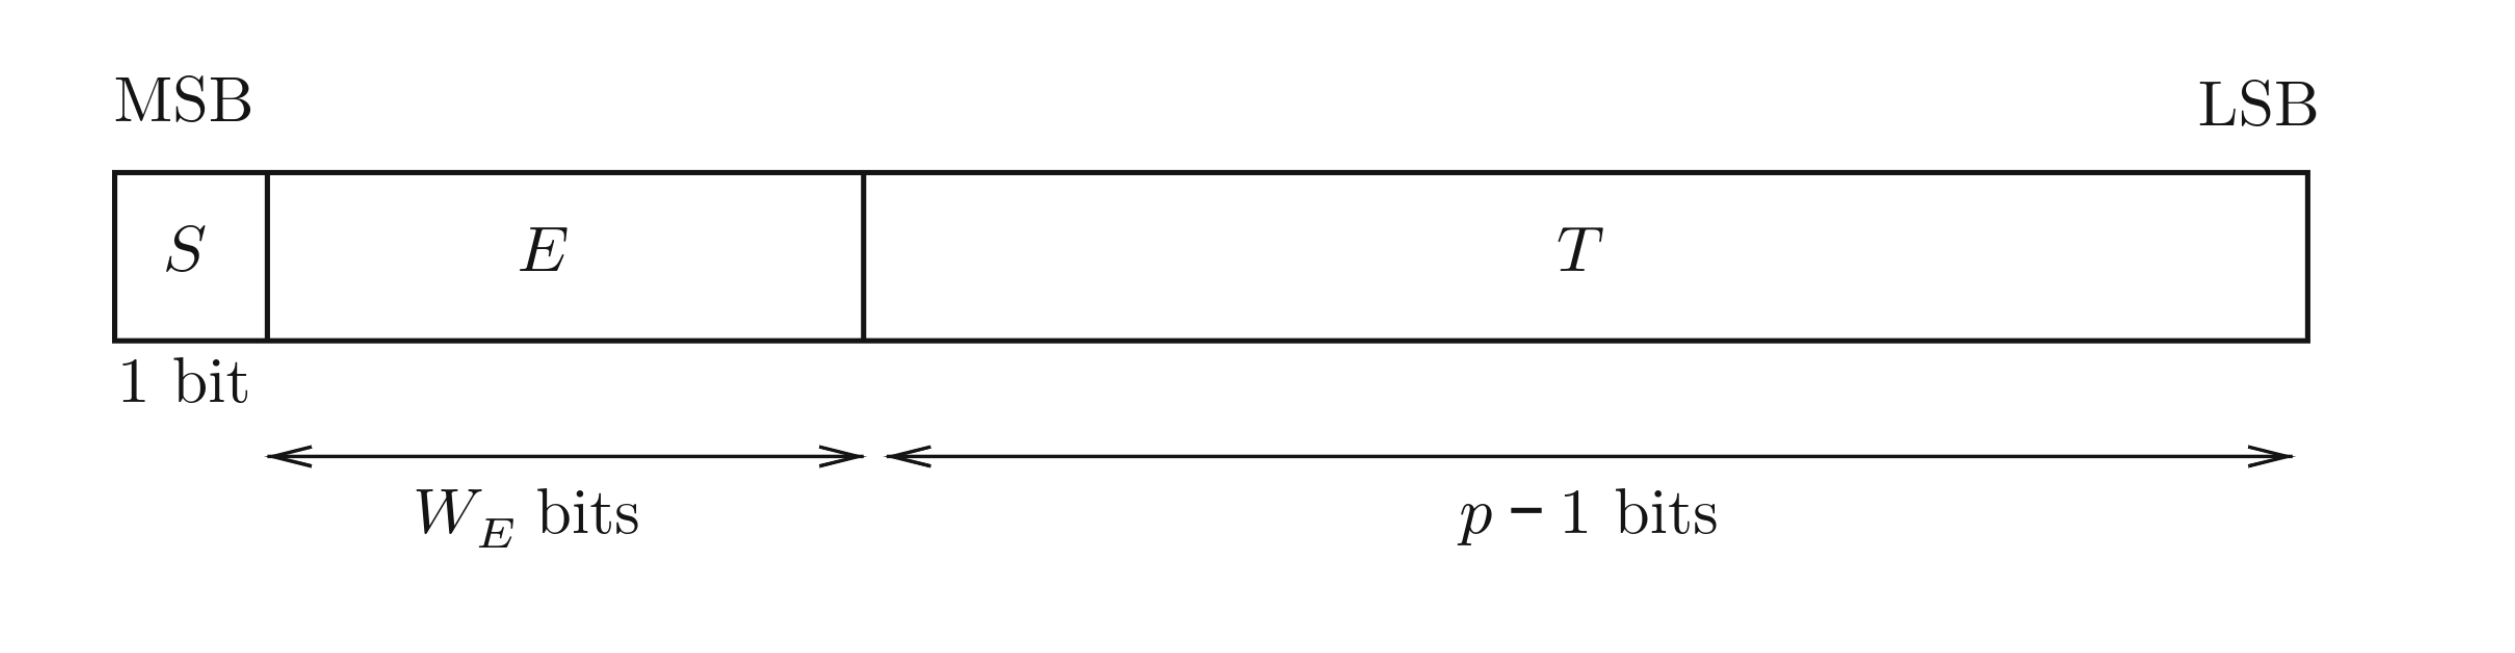
\includegraphics[width=\textwidth]{ieee754_binary_encoding.png}
	\caption{Encoding for the IEEE~754 binary floating-point formats}
	\label{fig:IEEE754-binary-encoding}
\end{figure}
				
\begin{table}[b]
	\centering
	\begin{tabular}{|l|c|c|}
		\hline
		Biased exponent $N_{e}$ &   
		% start 2nd col title
		\begin{tabular} 
		[c]{@{}c@{}}Trailing \\
		significand \\
		$t_{1}t_{2}\cdots t_{p-1}$
	\end{tabular} &
	% end 2nd col title
	Value represented \\ \hline
	$111\cdots1_{2}$      & $\ne 000\cdots 0_{2}$    & NaN                                                          \\ \hline
	$111\cdots1_{2}$      & $\quad 000\cdots 0_{2}$  & $(-1)^{s}\times\inf$                                         \\ \hline
	$000\cdots0_{2}$      & $\quad 000\cdots 0_{2}$  & $(-1)^{s}\times 0$                                           \\ \hline
	$000\cdots0_{2}$      & $\ne 000\cdots 0_{2}$    & $(-1)^{s}\times 0.t_{1}t_{2}\cdots t_{p-1}\times2^{e_{min}}$ \\ \hline
	$0<N_{e}<2^{W_{E}}-1$ & any                      & $(-1)^{s}\times 1.t_{1}t_{2}\cdots t_{p-1}\times2^{N_{e}-b}$ \\ \hline
	\end{tabular}
	\caption{Encoding to represent special values in the binary formats defined by IEEE~754-2008}
	\label{table:IEEE754-binary-encoding}
\end{table}
				
Representing the set of real number in a finite space is impossible; instead approximation is required.
The IEEE~754 formats have specified standard regarding rounding of inexact floating-points.
The following arithmetic functions are required to be correctly rounded: addition, subtraction, multiplication, division, and fused multiply-add (FMA).
The square root function and conversion between supported formats also need to be correctly rounded.
Additionally, the standard recommends a list of function to be correctly rounded. % TODO add reference to list of function (See page 79 of FP handbook)
% TODO Be more specific that this is for IEEE~754 when talking about correctly rounded function. Otherwise it can be confusing. Remove passive voice
There are three directed rounding attributes:
\begin{itemize}
	\item \textit{roundTowardPositive} $RD(x)$ rounds to the largest floating-point less than or equal to $x$.
	\item \textit{roundTowardNegative} $RU(x)$ rounds to the smallest floating-point greater than or equal to $x$.
	\item \textit{roundTowardZero} $RZ(x)$ rounds using $RD(x)$ if $x \ge 0$ or $RU(X)$ if $x \le 0$.
\end{itemize}
There are also two attributes for rounding to nearest, when a floating-point is exactly between two exact representations:
\begin{itemize}
	\item \textit{roundTiesToEven} $RN_{even}(x)$ rounds to the exact representation whose least significant bit is even.
	\item \textit{roundTiesToAway} $RN_{away}(x)$ rounds to the exact representation whose magnitude is the largest.
\end{itemize}
The standard for the binary formats requires the implementation of all three directed rounding and \textit{roundTiesToEven}.
				
While not a basic format, binary16 is starting to receive more attention and support as it is increasingly being used for computing application.
For example, it was found that some convolution neural network (CNN) perform well with binary16; and even with precision of only 8 bits \HL{{\cite{Muller2018-zm}}}.
Moreover, while most GPUs support both binary32 and binary64, more recent GPU architectures also support the binary16 format.
				
\section{Sources of error}
% TODO
% Merge with the section: defintion & basic notions.
% 1 page
\begin{comment}
- rounding & double rounding
- cancellation
- overflow & underflow
- accumulation
- swamping

%  Ask Yohan for further references
\end{comment}

\chapter{Reduced precision}
\label{ch:reduced-precision}
\HL{Computing applications are commonly developed to use the double precision.}
While this is necessary for specific applications, results obtained at a lower
precision are acceptable in many contexts.
As~\cite{Cherubin2020-tt} depicts, numerous studies explored the use of lower
precision data types to perform computations.
It is an interesting strategy as it has the joint potential to reduce hardware
size, energy cost, and execution time.
In this chapter, we present (1) the problem definition of \textit{Reduced Precision},
(2) various data formats used to perform reduced precision,
(3) methods to implement reduced precision,
(4) the growth of quantization in Deep Learning,
and (5) the benefits, limitation, and open questions of reduced precision.

\section{Problem definition}
\label{sc:rp-problem-definiton}
The IEEE~754 standard defines two main floating-point formats: FP32 and FP64.
However, not all types of applications require that much precision.
For this reason, many efforts were put into creating new data formats with lower precision (discussed in Section~\ref{sc:rp-data-format}).
The idea behind reduced precision is to represent numbers in a data format with
lower bit width, i.e., lower exponent or mantissa.
Similarly, mixed-precision is a concept that uses data formats of different precision within a program, allowing for better precision tunning.
The logic complexity of floating points is approximately proportional to the square of the bit width~\cite{Chen2018-an}.
Therefore, lowering the number of bits in a data format also reduces the die size
of a chip and, consequently, the energy cost and computation time for arithmetic operations.

The work in~\cite{Cherubin2020-tt} surveys a range of tools in the fields of reduced precision.
That same study defines five challenges that remain to be addressed for reduced precision:
\begin{itemize}
	\item[1.] Identify the code sections where applying reduced precision is beneficial;
	\item[2.] Determine the data type to use based on the application and architecture;
	\item[3.] Estimate, quantify bounds, and manage the numerical error introduced by applying reduced precision to an application;
	\item[4.] Measure the overhead from type casting between different data types;
	\item[5.] Develop a tool that benefits many applications and platforms.
\end{itemize}
The authors of this study claim that reduced precision will not be sustainable
in commercial or open-source applications without solving those limitations and
will mostly remain an academic subject.
Moreover, the current lack of tools to perform code conversion makes reduced precision
a significant development effort.
Overall, developing a tool that can be applied to multiple use cases and
architectures is an open issue~\cite{Cherubin2020-tt}.

\section{Data formats for reduced precision}
\label{sc:rp-data-format}
Although Chapter~\ref{ch:background} focused primarily on the IEEE~754 Binary data format, many other data formats exist.
This section introduces other data types used in reduced precision studies.

Common Deep Learning frameworks such as Tensorflow~\cite{tensorflow2015-whitepaper} and Pytorch~\cite{PyTorch_2019} support mixed-precision through their API.
Both frameworks support the classical IEEE float32 and float16 with the addition to the \textit{bfloat16} introduced by Google Brain~\cite{bfloat16}.
As shown in Figure~\ref{fig:bfloat16}, the bfloat16 is a 16-bit floating-point format that uses
the same number of bits as the IEEE float32 for its exponent while having shorter bit width for its mantissa.
\begin{figure}[b]
	\centering
	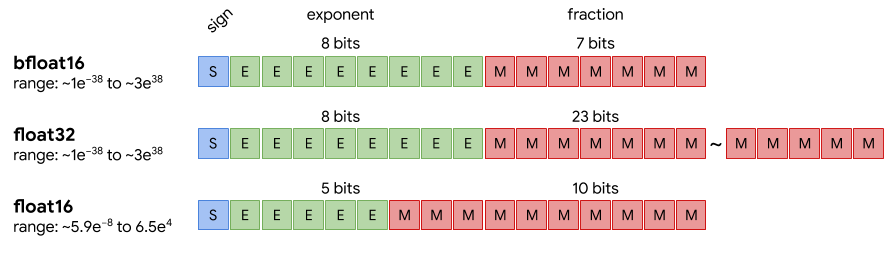
\includegraphics[width=\textwidth]{bfloat16.png}
	\caption{Representation of the bfloat16 format. (Taken from~\cite{bfloat16})}
	\label{fig:bfloat16}
\end{figure}
With the same exponent length as float32, bfloat16 allows for quick data type
conversions by dropping or adding the extra bits between float32 and bfloat16.
Moreover, with a smaller mantissa size, hardware chips for the bfloat16 multiplier
are about half the size of float16 ones and around eight times smaller than for float32~\cite{bfloat16}.
Additionally, since Neural Networks (NNs) are far more sensitive to the exponent range than the mantissa,
the bfloat16 performs well as it keeps the exponent range from float32.

Outside of standard Deep Learning frameworks, various data types were
studied to reduce the precision of machine learning models.
The work from~\cite{Johnson2018-up} evaluates a new \textit{posit tapered} data
format which combines ideas from the posit~\cite{Gustafson2017-wo} format and the log number system~\cite{Kingsbury1971-kx}.
Various other studies use different custom floating-point formats with reduced
exponent and mantissa size~\cite{Lesser2011-mn, Chen2018-an, Vicuna2021-mw, Wang2018-oo}.
The authors in~\cite{Carmichael2019-nu} designed three FPGAs for low-precision fixed-point, floating-point, and posit.

\section{Implementing reduced precision}
To remain efficient, consumer hardware only supports a limited set of data formats; for example, IEEE~754.
In addition, custom data formats often require specialized hardware, software implementation, or simulation. 

Implementing a new format can be tricky, with commodity hardware only supporting the most popular data formats.
A straightforward way to achieve this is to design custom specialized hardware capable of executing the new format.
The authors in~\cite{Carmichael2019-nu} designed three different FPGAs to support low-precision floats, fixed points, and posits.
Another study~\cite{Johnson2018-up} designed a \SI{28}{\nano\meter} ASIC to implement an 8-bit Exact Multiply-Accumulator (EMAC).
On the one hand, the main advantage of designing specialized hardware is efficiency.
Indeed FPGAs and ASICs designed for single tasks can be optimized much more than general-purpose hardware.
For example, major hardware manufacturers such as Nvidia, Google, and Intel
design specialized hardware for frequent Deep Learning tasks (GEMMs) with their
recent GPU architectures and TPUs~\cite{tpu,intel-BF16-2018}.
On the other hand, creating new hardware is costly in time and material.
This is especially true when performing a study that evaluates a range of different data formats.

Since hardware implementations can be challenging, some research investigated
software solutions to implement reduced precision.
In~\cite{Anderson2016-yn}, the authors proposed a new data format, \textit{flyte},
with a mantissa that differs in 8-bits increment from the traditional IEEE~754
standard while keeping the exponent the same.
This allows native instructions to read data with power-of-two bit width.
The authors suggest a packing and shuffling method to prevent cache miss due to misalignment by reorganizing the flyte in the vector registers.
However, some issues with misalignment for some flyte formats resulted in a lower performance gain.
Overall, their technique significantly reduces cache misses for \textit{BLAS} Level 2 and 3; as many as $4.5\times$ less than double precision.
The authors in~\cite{Zucker1994-rg} propose an algebraic method to pack multiple
low-precision operations into a single high-register operation.
This method showed a performance improvement of 8.7\%, 13.6\%, and 16.2\% when packing
2, 4, and 8 numbers, respectively.
Unfortunately, this technique can only be applied to a few algebraic operations.
On the one hand, software implementations are less efficient than specialized hardware
since they suffer from substantial overhead costs.
Often, implementing software solutions requires high manual efforts, whether to
perform code conversion or design a new data format.
On the other hand, software design can be more portable across architecture than specialized hardware.

As an alternative to hardware or software implementation, a common approach to
prototype or study new data formats is through simulation.
The work in~\cite{Chatelain2019-fu} explores reduced precision to lower the communication costs of iterative methods.
They use the VPREC backend in Verificarlo to simulate reduced precision combined
with a heuristic to determine a minimum precision for the different iterations.
They consider both temporal and spatial changes in the precision of applications.
Other studies~\cite{Higham2019-yd,Zhang2019-xv} propose simulation methods for reduced
precision on single operations and kernels.
The work in~\cite{Higham2019-yd} implemented a reduced precision library in MATLAB, and
the work in~\cite{Zhang2019-xv} developed a high-level framework on top of PyTorch to use
reduced precision techniques.
The main benefits of simulating reduced precision are the low implementation cost and new hardware not needing to be designed.
This often allows exploring a large number of data formats with fewer efforts.
Unfortunately, while simulations are great for accuracy evaluation, it is still challenging to simulate performance due to the complexity of modern systems.
Moreover, simulating reduced precision comes at a substantial overhead cost.
Therefore, it is required to implement a hardware or software implementation later to achieve performance.

\section{Quantization in Machine Learning}
In recent years, machine learning, and more specifically Deep Neural Networks (DNNs),
have seen a rise in popularity due to their ability to solve challenging problems.
However, the complexity of DNN models comes with a high usage of computing resources.
With the enormous datasets required to train these models, compute and data communication time is usually a bottleneck.
This motivated multiple studies \cite{Johnson2018-up,Wang2018-oo,Lesser2011-mn,Chen2018-an,Judd2015-kw,Vicuna2021-mw}
to explore the possibility of reducing the precision of the data format used to train those models.
This section explores the quantization methods developed in the Deep Learning domain to reduce models' computing and data communication.

The authors from multiple studies explored the effects of quantization for SVM classification
and found it possible to use minimal precision without accuracy loss.
In~\cite{Lesser2011-mn}, the authors investigate the impacts of reducing precision for SVM
classification and estimate the minimal precision required to achieve classification
without loss of accuracy. They performed three experiments:
(1) adding noise to parameters,
(2) using MPFR, simulating reduced mantissa precision from 53 to 4 bits,
and (3) combining the experiment (1) and (2) concurrently.
By comparing the effects of quantization with and without rounding, it is possible to isolate better
the impact of rounding due to reduced precision.
The authors benchmark their experiments on three datasets: SONAR, IRIS, and MUSK.
They use the double precision results as a reference for the classification error.
The results show that lowering the precision up to 15 bits does not affect the accuracy
for classification.
Further understanding the bounds for reducing the precision would allow to automatically
adjust the precision for classification, which would be an effort towards addressing the third
challenge from Section~\ref{sc:rp-problem-definiton}.

With the increasing complexity of  DNNs, it becomes difficult to train the models with
techniques to improve performance, such as data sampling or model parallelism.
It is also problematic to integrate those models into embedded systems due to resource limitations.
While many studies found that CNNs are resilient to accuracy loss when using reduced precision,
few of them attempted to vary the precision used at each layer.
The authors in~\cite{Judd2015-kw} show that the precision required in different layers and networks differ significantly.
Moreover, they suggest a method to select the appropriate precision of each layer while
keeping accuracy within a determined boundary.
Their model converts floating points to the appropriate representation and then back to single-precision after processing a layer.
To evaluate their method, the authors benchmark their reduced precision model on five popular CNNs.
Through their experiments, they reduce the precision of both the model's weights and the output of each layer.
Their first experiment reduced the precision of all layers simultaneously in the range of 12 to 1 bits.
The results show that only 21 bits would be required to store both the weight and output data of a layer.
Next, the authors reduced the precision of individual layers to obtain the importance of precision for each layer.
From the results, we observe that the precision required by each layer varies significantly.
The authors also calculate an estimated data communication for the networks.
Finally, they also propose a method to find the minimal precision per layer while preserving accuracy:
\begin{itemize}
	\item[1.] Set the layers to an initial uniform precision with less than $0.1\%$ error.
	\item[2.] Create a collection of deltas by reducing the precision of parameters and layer output by 1 bit for each layer.
	\item[3.] Use the configuration with the best accuracy for the next iteration.
\end{itemize}
To find the best mixed-precision, although potentially sub-optimal, the authors use a Pareto
frontier between the amount of data transfer and the accuracy for different configurations of bit precision.
Although sub-optimal, this heuristic resulted in an average decrease of $74\%$ of data traffic
while preserving accuracy within $1\%$ of tolerance.
This work shows the potential of using various precision sizes for different layers of CNNs.
Furthermore, it motivates further efforts to study strategies in further exploiting reduced precision to reduce memory usage and compute time.

Linear algebra operations are critical components in most DNNs models such as
the multiply-accumulate (MAC) operation ($\sum_{i}a_{i}b_{i}$).
The authors in~\cite{Johnson2018-up} describe \textit{ELMA}, a new method to compute MAC using a combination of the logarithmic
number system~(LNS), \textit{Kulisch accumulator}~(EMA), and the posit data format~\cite{Gustafson2017-wo}.
The authors evaluate the accuracy using an FPGA implementation of the ResNet-50~ImageNet model.
Moreover, the new ELMA implementation is compared in the area~($\SI{}{\micro\metre}^2$)
and power~(\SI{}{\micro\watt}) using a \SI{28}{\milli\metre} ASIC library.
The results show that the proposed ELMA operator reduces the power usage on
multiplications by \SI{90.9}{\micro\watt} but increases it for additions by \SI{68.3}{\micro\watt}.
Overall, the net power usage is lower than in previous methods suggesting that
further efforts to reduce floating-point efficiency could bring substantial benefits.

Without a doubt, DNNs emerged as a powerful tool to solve problems.
However, to achieve high accuracy, DNNs require a tremendous amount of resources;
with models reaching 100s of \SI{}{\mega\byte}s, and computation on large datasets can span multiple days/weeks.
In~\cite{Chen2018-an}, the authors explore approximate computing to reduce both 
computation and data communication of DNNs, while preserving accurate results.
The authors quantize the weight and activation of the model from 16 to 2 bits.
Then, the authors benchmark the reduced precision model on four popular DNNs to evaluate its accuracy.
They find that at 4 bits, the accuracy remains within $<1\%$ of the reference
full-precision model while improving performance by $4.5\times$.
When reducing the precision of the models to 2 bits, the authors achieve a $14\times$
improvement in normalized chip density, resulting in lower energy consumption.
Overall, the results from this paper show promising benefits to further studying
reduced precision strategies as it jointly reduces hardware and energy cost and
computing and data communication time. 

Numerous approximate computing methods have been studied for deep learning to
reduce computation and data communication time and energy cost.
The energy efficiency of hardware approximately increases quadratically with the reduction in bit precision~\cite{Wang2018-oo}.
With current hardware implementing 16 bits of precision, we can see performance improvements of $\ge 4\times$ compared to 32 bits.
Studies showed that the computation steps for DNNs inference could be reduced to as low as 2-4 bits
while remaining accurate, and even precision of 1-2 bits for weights and activations.
However, an empirical study found that a precision of 16 bits was required during
DNNs training to preserve accuracy.
When trying to reduce the precision further, DNNs often start to see significant
accuracy degradation, issues with convergence, and an impact on overall accuracy.
The authors in~\cite{Wang2018-oo} suggest using \textit{FP8} combined with 
\textit{chunk-based computations} and \textit{stochastic rounding} to further reduce
the bit precision compared to state-of-the-art methods while maintaining accuracy.
They evaluate their methods on a collection of 6 NNs models across multiple datasets.
The results show that their implementation using both FP8 and FP16 is equivalent
in accuracy to FP16 and FP32 while performing $2-4\times$ faster.
Moreover, the authors found that keeping a higher accuracy (FP16) on the first layer~(input data)
and the last layer was critical in training their FP8 models successfully.
This work shows that effort in reducing floating-point precision in deep learning
can increase performance significantly while keeping accuracy equivalent.

While machine learning models are a great tool to solve problems, they can be challenging
to implement on embedded systems due to their large memory requirement.
Mondrian Forest, an online classifying algorithm, is typically too memory-intensive
for embedded devices; therefore, using reduced precision could enable its use.
The authors in~\cite{Vicuna2021-mw} explore reduced precision techniques on Mondrian Forests
to reduce their memory usage.
They study the model parameters, numerical precision, and memory consumption together
due to their interdependence.
Using VPREC, the authors simulated reducing the bit precision $p$ from 52 to 1 bit.
Moreover, the exponent range is varied from 11 to 2 bits.
The model is instrumented both at a node level and for the whole model.
To evaluate their method, they use two publicly available datasest: Recofit, and Banos et al.
To quantify the model's performance with different memory constraints, the authors allocate three
different values of memory limit for the model: \SI{0.6}{\mega\byte}, \SI{1.2}{\mega\byte}, and \SI{3}{\mega\byte}.
Their results for node instrumentation show that for $p \ge 2$ the F1 scores remain with a standard deviation.
However, the F1 scores are significantly different for the complete instrumentation when $p \le 6$.
The observations on the F1 scores for $p > 2$ were not correlated to memory.
This suggests that using reduced precision with different memory allocations would yield similar results.
Given constant memory constraints, the authors found that reducing precision allows the
trees to grow deeper, potentially improving the classification performance.
Overall, the results show that Mondrian Forest can be implemented with an 8-bit floating-point
format without affecting the F1 scores significantly, which has the potential to
reduce memory footprint by roughly $1.8\times$ compared to double precision.

Although Section~\ref{sc:rp-data-format} discussed reduced and mixed precision
in popular deep learning frameworks like PyTorch and Tensorflow, the scope of
ultra-low precision (i.e., $\le 8$ bits) is still a topic limited to academia.
Further efforts are required to understand better the effects of reduced precision 
on different models and datasets; without it, the reach of ultra-low floating-point will remain restrained.
Furthermore, while the deep learning community has vastly explored reduced precision
techniques to the best of our knowledge, the topic remains unexplored in most other fields of application.

\section{Discussion}
\label{sc:reduced_precision_discussion}
In this chapter, multiple studies showed promising reduced precision approaches
to improve the performance of applications while preserving accuracy.
However, reduced precision comes with its caveats.
We will discuss the benefits and limitations of using reduced precision throughout this section.
Moreover, we will discuss open problems in the field of reduced precision.

By reducing the number of bits used to represent numbers, the memory footprint
of applications is directly reduced.
This has two main benefits: applications require fewer resources to execute, reducing the hardware cache miss, which increases performance.
Additionally, reducing the size of the data format allows specialized hardware
or software techniques to pipeline operations together.
With hardware complexity being approximately proportional to the square of the
number of bits~\cite{Chen2018-an}, reducing the data format can jointly increase
performance and reduce energy costs.
Furthermore, fusing multiple low-precision data format operations in a single register operation can lower computational costs. 
Lastly, reducing the size of input and output data would lower storage space requirements.

Using reduced precision requires substantial efforts for creating, evaluating, and implementing new data formats.
\HL{This is amplified by the current lack of understanding of the effects of applying
reduced precision to various applications and, in general, the precision required for a specific application.}
Even within a single application, varying the data can substantially modify the
precision required to preserve accurate results.
Finally, the conversion between data formats comes with an overhead cost.
Thus, attention must be paid to minimizing the amount of data format conversions
within an application when applying reduced precision.
Otherwise, the performance benefits from using reduced precision might be overtaken
by a high overhead cost in data conversion and result in an overall slowdown
in the performance of an application.
\HL{
	While hardware is an efficient way to implement reduced precision, it is also costly
	in time and material.
	On the opposite, software implementation is less efficient but tends to be more portable.
	Lastly, simulating reduced precision has a low implementation cost and does not
	require specialized hardware; however, it is limited to prototyping new data format and requires
	either a software or hardware implementation to improve performance.
}

To have a broader adoption of reduced precision, some critical limitations need to
be addressed, including but not limited to:
\begin{itemize}
	\item Determine the different sections of code that can take advantage of reduced precision
	      while considering both temporal and spatial variability of precision.
	\item Improve the heuristics for finding the minimal precision required for each code section.
	\item Estimate the performance gain from using reduced precision.
	\item Understand the effects of reduced precision when varying the data in an application.
	\item Automate the code conversion to simplify the usage of reduced precision.
\end{itemize}
To the best of our knowledge, these problems remain open challenges within reducing precision.
Therefore, further research will be needed to make progress in resolving these challenges.

\chapter{Neuroimaging applications}
\label{ch:neuroimaging}
To study the brain and diagnose patient in clinics, the neuroimaging community
developed multiple ways of capturing, processing, and analysing brain data.
This chapter discuss the three important magnetic resonance imaging (MRI)
modalities for neuroimaging and associated pipelines to processed them, more
recent machine learning techniques for neuroimaging, and discuss the potential
of using reduced precision techniques for neuroimaging tools.

\section{MRI processing}
\label{sc:preprocessing}
Magnetic resonance imaging (MRI) is a common tool used by neuroscientist to perform clinical
diagnosis and for researchers to gain a better understanding of the brain.
With the evolution of MRIs, three main modalities emerged: structural MRI, 
functional MRI (fMRI), and diffusion MRI (dMRI).\
While other modalities such as EEG, CT, and PET exist, we focus on MRI data types
for their non-intrusive property.
Additionally, MRI analysis are technically challenging to process due to the complexity
of the pre-processing steps involved and the large data size produced as output 
and during intermediary steps.
In this section, we briefly introduce these different MRI modalities.
Moreover, we will explore relevant preprocessing steps to analyse the data and 
describe standard software toolkit to perform the preprocessing and analysis for
each modalities.

Structural, or anatomical, MRI is a classical method that is vastly used in clinical diagnosis.
The aim of structural MRI is to provide static information on the anatomy of the brain.
With the use of T1-weighted and T2-weighted images, it allows the diagnosis and 
monitoring in applications such as: epilepsy, Parkinson's disease, acute 
cerabral haemorrhage, and multiple sclerosis~\cite{Symms2004-xj}.
Capturing data accross different individuals, sessions, or even scanner types will
oten result in a significant variation of brain structure.
To perform a meaningful analysis it is required to realign the data into
a common space; thus reducing variability.
Two popular methods are \textit{volume-based normalization}, which uses a
template to realign an image to the common space, and \textit{surface-based normalization},
which takes advantage of the fully connected topology of the cerebral cortex to
normalize the surface of the brain tissues.
Other preprocessing steps that are standard for anatomical data are \textit{bias field correction}
to correct the variation in voxel intensity, \textit{brain extraction}, and \textit{tissue segmentation}
to seperate the different components such as gray matter, white matter, and cerebrospinal fluid.
FreeSurfer~\cite{Fischl2012-bp} is a toolkit that allows the preprocessing and analysis of structural MRI.
Amongs it's many feature, it implements accurate topology correction, surface-based inter-subject alignment,
volume and surface cross-subject registration, and whole-brain segmentation.

Unlike structural MRI, fMRI is used to measure the brain activity and connetivity.
fMRI became dominent due to its fundamentely non-invasive acquisition, high spatial
resolution, signal reliability, robusteness, and reproducibility~\cite{Soares2016-tz}.
The measurements of fMRI data is based on the concept that neural activation involves 
an augmentation in blood flows.
It capture images of the brain using the blood oxygenation level-dependent (BOLD) contrast methods.
Figure~\ref{fig:fmri_workflow} depicts the major preprocessing steps to correct 
for artifacts in the data prior to analysis.
Head motion is a critical issue during fMRI acquisition.
To correct for it, a common strategy is to use a reference volume to realign the data.
Spatial transformation is required to analyse the subject in the same space.
For this step, the volumes are normalized to an template.
The different sections of brain data are acquired at different slices.
To perform proper analysis, the data from the slices needs to be corrected to interpolate
the signal at a certain time point.
Another important step is spatial smoothing, which average the data points with their neighbors.
This increase the signal to noise ratio for the data and improve the results of statistical tests.
Multiple techniques were developped to perform statistical analysis on the 
preprocessed data of task-based and resting-state studies.
fMRIPrep~\cite{Esteban2019-og} is a toolkit that offers various techniques for the preprocessing steps 
and statistical analysis of both resting-state and task-baseed function MRI data.
The pipeline dynamically assemble sub-workflow that best suit the data for preprocessing.
Additionally to the data output, it creates a HTML report for users to asses the quality of the data generated.
With a joint combination of a citation boilerplate, thorough documentation, and open-source code
fMRIPrep implementation and processing is transparent and encourage reproducibility.

\begin{figure}[h]
	\centering
	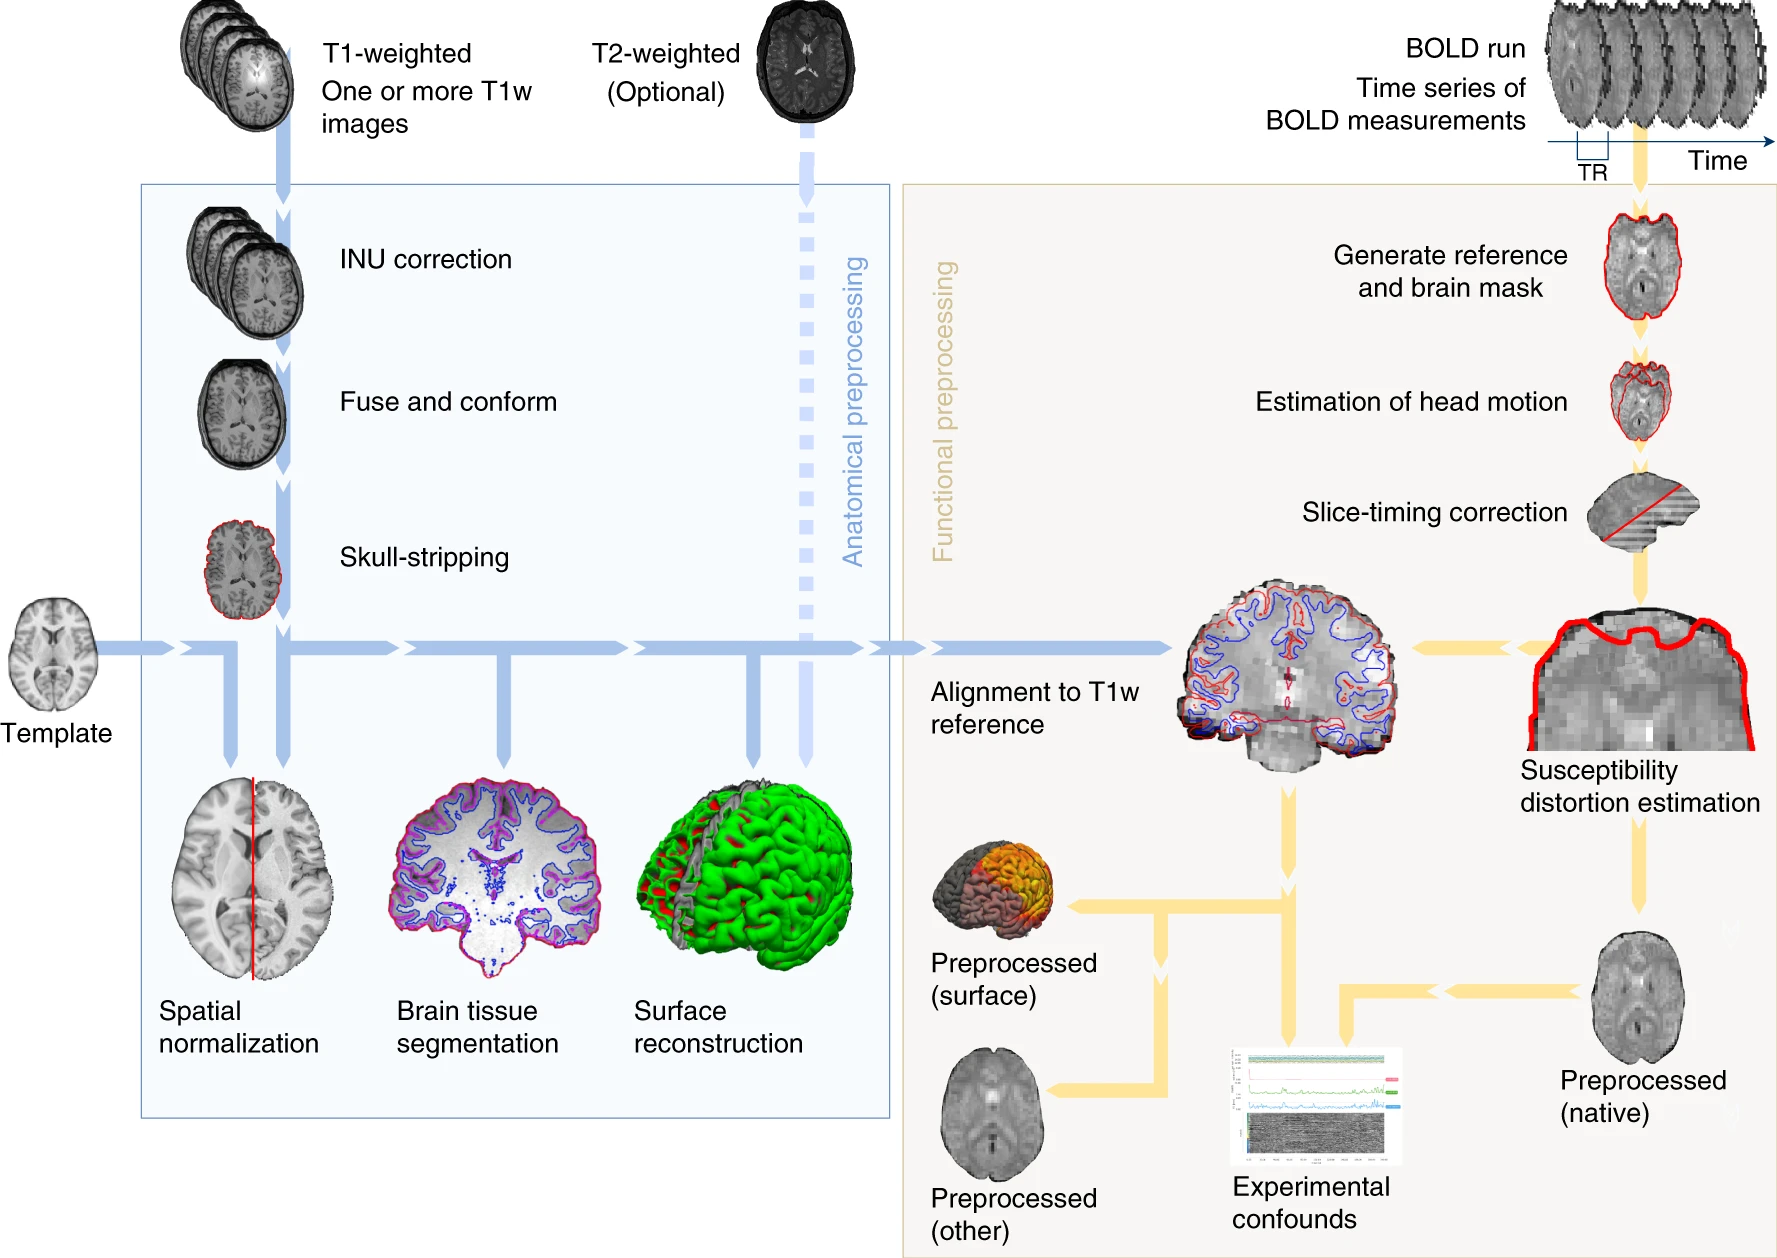
\includegraphics[width=\textwidth]{fMRIPrep_workflow.png}
	\caption{Preprocessing steps for structural and functional MRI data. (Taken from~\cite{Esteban2019-og})}
	\label{fig:fmri_workflow}
\end{figure}

While fMRI uses BOLD signal to capture data, dMRI exploits the magnetization of hydrogen in water molecules.
The water molecules diffuse at different rates depending on the tissue types, 
integrity, and architecture giving information about its direction and anisotropy~\cite{Soares2013-hw}.
This makes dMRI more suitable to study the neuronal function than blood-flow-based approach such as fMRI.
For example, to map brain connection or detect faulty connection of some psychiatric disorders~\cite{Le_Bihan2015-vp}.
Just like structural and functional MRI, dMRI acquisition is very sensitive to motion.
Correcting head motion is required during preprocessing.
Optionally, skull striping can also be performed to extract the brain data for analysis.
Dipy~\cite{Garyfallidis2014-ve} is a toolkit to perform these preprocessing techniques
on dMRI data and offers different modules to perform analysis and visualization of data.
Moreover, Dipy is integrated within the neuroimaging Python ecosystem.

The different MRI modalities presented in this section offer a non-intrusive way to study the brain.
However, they require multiple complex preprocessing steps before doing analysis of the data.
Lastly, a multitude of mature toolkit for preprocessing and analysis exist to process MRI data.


\section{Machine Learning applications} % 2
In recent years, machine learning (ML) methods have seen an increase interest 
accross multiple fields of application; neuroimaging is no exception.
While most ML techniques for neuroimaging lays in the analysis stage, some recent 
work tackle the problem of pre-processing using Deep Learning (DL).
Throughout this section, we will review some of the ML methods for analysing MRI 
data, their heavy usage motivating the development of a specific machine learning
framework for neuroimaging analysis, and recent work that use DL techniques to 
speed up current neuroimaging pipelines.

Using machine learning techniques to perform neuroimaging analysis is challenging.
Inherently, neuroimaging data contains few subjects (samples) and very large amounts
of voxels (often used as features).
The author in~\cite{Davatzikos2019-dc} says that, as of 2019, ML techniques used in
neuroimaging are not mature enough to be reliable in application.
However, a lot of efforts are put to overcome the current challenges in the field.
In a recent study~\cite{Mateos-Perez2018-wx}, the authors review ML applications on MRI data,
mainly structural, for both predicting clinical status or finding regions of interests (ROI)
for diseases and disorders.
Some of the applications presented include, but are not limited to: 
classification of Alzheimer's disease, diagnosis of Autism, automatic segmentation
of white matter lessions, or classification of the differents stages of Parkinson
and combinations of diseases with similar symptoms.
While obtening high accuracy is objectively desirable, in neuroimaging, it is much
more important to understand what are the major factors that influenced in making a prediction.
That is, understanding which features impact the prediction of some disease helps
in gaining knowledge on their biological implications.
This in part might explain the predominance of SVM in the analysis of neuromaging studies.
While ML methods are still growing in neuroimaging, they are invaluable in gaining 
a deeper understanding of the underlying biological aspects of diseases and disorders.

The joint combination of the increased prevalence, multiple methods, and unique 
challenges of machine learning methods in neuroimaging, motivates the development
of specific tools to perform ML analysis for neuroimaging.
The authors in~\cite{Abraham2014-zv} discuss the main steps performed for some 
neuroimaging analysis while using ML techniques.
In the same paper, the authors describe the main constructs used to develop
\textit{Nilearn}: A statistical analysis framework for neuroimaging in Python.
To name a few, Nilearn facilitates the steps to perform analysis by offering 
methods to perform data preparation such as reasmpling, signal cleaning, or data
visualization, decoding and encoding tools, and resting-state and functional connectivy analysis.
While such frameworks offers a multitude of tools to perform statistical analysis,
they still require pre-processing of the data, which is computatively demanding.

Thus far, the ML methods for neuroimaging that we discussed were only classic 
statistical methods, however, multiple DL techniques have also been studied.
In a recent review paper~\cite{Wen2018-to}, the authors discuss three applications
which can benefit from DL models.
In one paper reviewed~\cite{Nie2016-sw}, using features extracted from a CNN,
a SVM classified the lifetime of patients with brain tumors.
In another study~\cite{Wen2018-xm}, fMRI data related to data is interpreted using an auto-decoder.
Lastly, in~\cite{Zou2017-hd}, a 3D-CNN is used to classify ADHD.
While showing showing promising accuracy and fast inference time, training DL models
requires extensive training time and is prone to over-fitting; especially in the
setting of neuroimaging where the number of sample is low.

Two distinct parts of neuroimaging computing is the pre-processing steps and the analysis.
So far in this section, we only discussed the ML methods used for analysis due to
the large amount of studies using ML to perform neuroimaging analysis.
While few, there are some emerging efforts that propose using DL methods to speed up
the computation of the pre-processing steps.
With claisscal pre-processing pipeline being compute and time intensive, using 
DL techinques could significantly reduce the pre-processing time of neuroimaging studies
and bring more applications in clinics which requires results in a timely manner.
This motivated the development of FastSurfer~\cite{Henschel2020-vq}.
The authors of this framework develop novel methods to perform fast volumetric segmentation,
reconstruction of the cortical geometry, and estiamte the morphology of the brain.
While other tools use DL to solve specific problem of the pre-processing pipeline,
FastSurfer is a whole framework that allows complete pre-processing replicating the 
FreeSurfer framework.
The authors claim that ``despite being despite being orders of magnitude \textit{faster} than
traditional approaches, FastSurfer increases \textit{reliability and sensitivity}'' compared to FreeSurfer.
FreeSurfer generally takes \SI{7}{\hour} for a complete pre-processing pipeline, while
FastSurfer only takes approximately \SI{3.7}{\hour}; with only \SI{1}{\minute} of
processing time required to perform volumetric segmentation for both the cortical and subcortical regions.
This introduce the potential to perform studies on larger datasets and enables more
applications where segmentation processing time is needed.

With the many efforts put into developping ML techniques for neuroimaging, they 
became an intrisic part of the field.
The numerous applications and the complex challenges related to neuroimaging 
motivated the development of frameworks specific to the domain, such as Nilearn.
Furthermore, more recent work use DL models to increase either, or both, of accuracy
and processing speed for pre-processing and analysis.
While some challenges remain, the current integration of ML models into neuroimaging
shows promising results for better understanding of the biological implications from 
brain activation, coducting study on larger datasets, and increase the 
applicatibility where results are needed imminently.

% TODO Rephrase the: to find about biological implication. More to understand feature importance ➝ explainable AI.
% TODO Change the sentence on SVM. SVM are good when having small datasets. Not sure if they are strong for being explainable.
% TODO Explain more on the features used for ML in neuro.

\section{Reduced precision for neuroimaging} % 1-2
With the joint combination of complex pipelines and large datasets in the field 
of neuroimaging, the question arise as wether or not reduced precision techniques
could bring performance improvements to the field.
In this section, we discuss the current reduced precision work for neuroimaging,
the state of numerical stability in neuroimaging pipelines, and some commonly used
techniques in neuroimaging pipelines that have similar effects as reduced precision.
\MD{TODO: a bit repetitive, try to remove some of the neuroimaging terms.}
	
\subsection{Current work}
To the best of our knowledge, only a few studies applied some form of reduced precision
techniques in neuroimaging; we present these studies here after.
Nguyen et al.~\cite{Nguyen2018-lo} present an empirical-Bayes false discovery rate
control method, to reduce the false positive results from concurrent hypotheses 
when only the p-values or test statistics are available; and those are stored at reduced precision.
In their study, they consider integer compression for 8 and 16 bits.
The results show that their method is on par with other state-of-the-art methods.
	
Performing whole brain segmentation is a challenging task, which usually requires
some division-and-aggregate techniques~\cite{Li2021-rv}.
By consequences, multiple passes need to be done and the results are estimated from
sampled region, therefore affecting both performance and accuracy.
The authors in~\cite{Li2021-rv} propose a whole brain segmentation techniques 
using mixed-precision (16 and 32 bits) on GPUs.
This allow both fast computing and the use of full volumes for training.
Their results depicts that inference time, for the segmentation, is around 200 times faster
than other methods (FCN~\cite{Long2015-qr}, U-Net~\cite{Ronneberger2015-wy}, and FastSurfer~\cite{Henschel2020-vq}).
Moreover, the results suggest that training the model with higher resolution volumes
improve the model generazability.
	
3D image registration is yet another fundamental and computationally expensive part
of neuroimaging pipeline.
Traditional methods take a few minutes to perform an image registration on CPU.
For large studies with thousands of subjects, improving this process has the potential
to lower computation time from weeks to days.
Brunn et al.~\cite{Brunn2021-zj} introduce a new method to perform image registration
using optimized mixed-precision code on GPUs and substituting 8th order finite difference
derivatives in-place of FFT-based first order ones.
Their results show a 30x performance and 6x mismatch improvement in comparison to 
another state-of-the-art pipeline (CLAIRE~\cite{Mang2019-nu}).
	
In general, the studies in which reduced precision was applied to neuroimaging 
do not have reduced precision has the main focus.
They only use it in combination of a primary suggested method.
Henceforth, there is currently a lack of understanding of the behavior and limitations
that reduced precision has on the field of neuroimaging.

\subsection{Challenges and Opportunities in Neuroimaging}
While applying reduce precision techniques to neuroimaging pipelines seems to be a
good idea, limited studies have done it thus far.
Here below, we discuss the potential challenges and opportunities to implement
reduced precision in the field of neuroimaging.

Inherently, evaluating the correctness of neuroimaging pipelines is challenging due
to the lack of ground truth from results of analysis.
That is, different pipelines can produces different results yet all be valid.
Neuroimaging applications often fit algorithm using low amounts of sample with variable
signal-to-noise ratio, which can potentially lead to instability when minor pertubations are applied~\cite{Kiar2020-uv}.
Li et al.~\cite{Li2021-om} studied the inter-pipeline variability while using the same data.
They found that there was a lack of agreement between pipelines and the steps leading
to those variability varied across pipelines.
When using test-restest data, they found that varition within small datasets have 
a larger impact on variability than inter-pipeline agreement.

In neuroimaging, numerical stability can arise from different sources including
acquisition noise, flexibility of the methods, and the pipelines used to process the data.
Salari et et al.~\cite{Salari2021-kd} studied the impact of operating system update on
the numerical stability of neuroimaging pipelines.
Using \textit{fuzzy libmath}, an extension to Verificarlo, they varied the virtual
precision of a preprocessing pipeline from 53 to 1 bits in increment of 2.
Moreover, they evaluated the stability of the pipeline accross a range of different 
operating system version; each using a different glibc (mathematical library) version.
Figure~\ref{fig:salari2021_vprec} suggests that increasing the precision above 21 bits
would not increase the numerical stability of the resutls from the pipeline.
\begin{figure}[h]
	\centering
	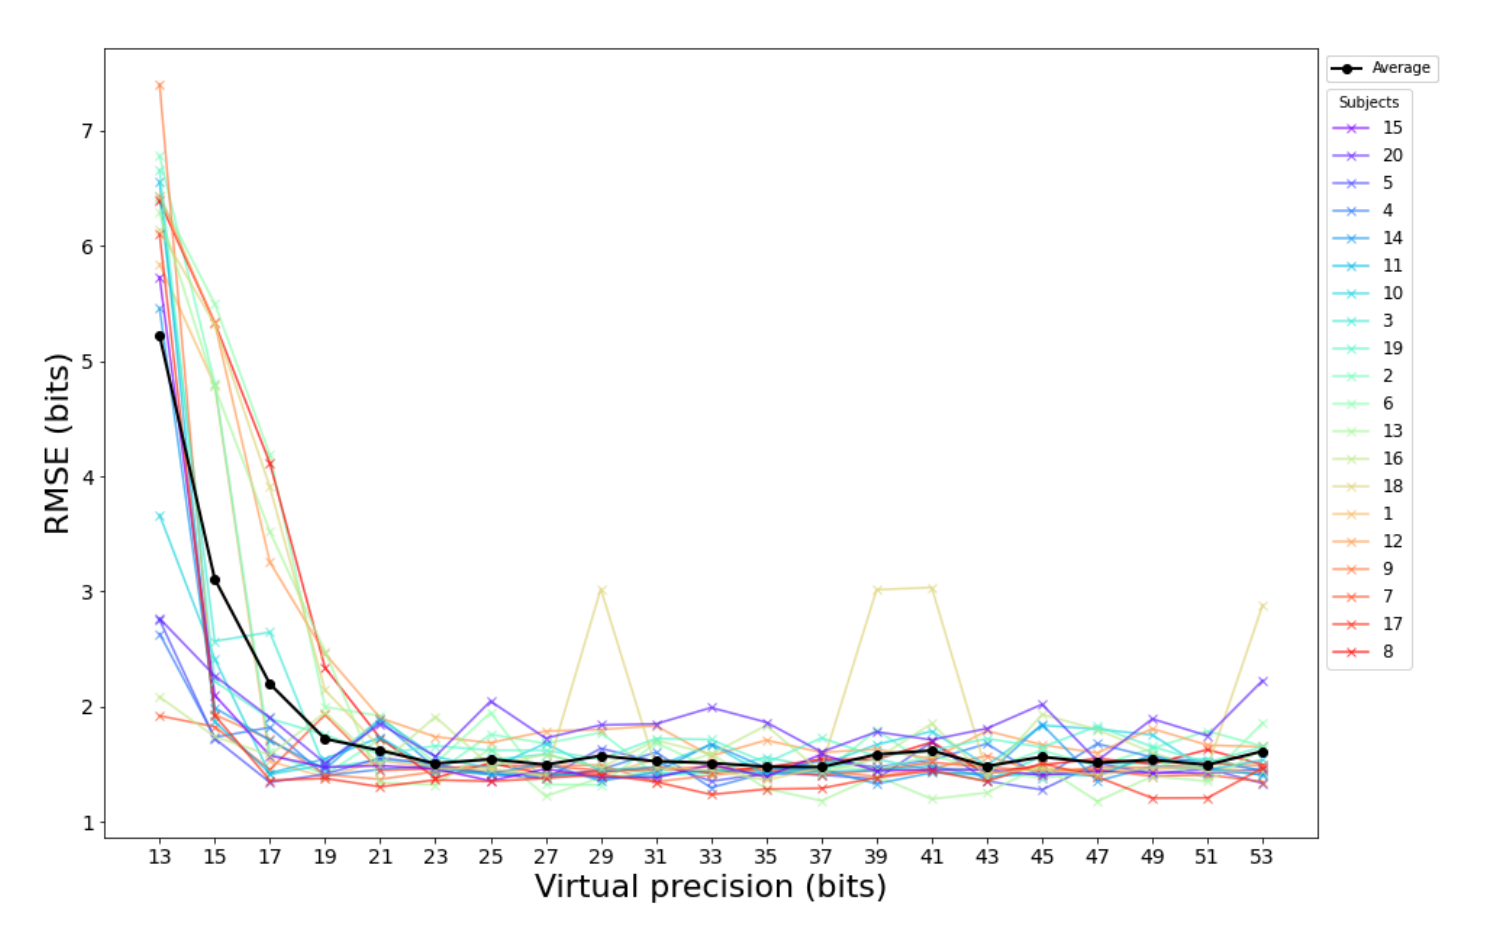
\includegraphics[width=\textwidth]{salari2021_vprec.png}
	\caption{RMSE values between OS and fuzzy libmath at each virtual precision.}
	\label{fig:salari2021_vprec}
\end{figure}

Image smooting is a commonly used method in neuroimaging pipelines.
It reduce the resolution of the data by combining close by voxels together.
Although in different ways, both image smoothing and reduced precision will affect
the precision of the data processed.
In a study by Molloy et al.~\cite{Molloy2014-oc}, the signal-to-noise ratio and the detection power
of fMRI signal could be improve by image smoothing, which is consistent with the literature.
Moreover, they found that applying spatial smoothing did not significal change the
results for functional connectivity when finding ROIs.

While image smoothing helps in correcting artifacts such as head motion, the smoothness
might be varied across the brain volume.
This can lead in confounds related to the smoothing of head motion.
Scheinost et al.~\cite{Scheinost2014-ds} propose a uniform spatial smoothing method
to reduce those confounds.
The authors found that uniformly smoothed volumes results in significanlty lower
correlation between regions and head motion.
Similarly to other smoothing techniques, it was not able to remove all confounds, however,
it remains promising.

Overall, while some studies show concern about the numerical stability of neuroimaging
pipelines, others suggests that a low amount of significant bits are used to perform calculations.
Moreover, frequently used smoothing techniques reduced the resolution in similar fashion
that reduced precision would.
Additional research is needed to better understand the effects of applying reduced
precision to neuroimaging pipelines.

\chapter{Conclusion}
\label{ch:conclusion}
With the increased interest in reduced precision in machine learning, we are interested
in exploring if its applicability could benefit other fields, particularly neuroimaging.
Firstly, we presented the fundamental notions about floating-point, defining the representation
of numbers as floating-point and the hidden bit convention that exploits some characteristics
of floating-point numbers.
Moreover, we explained the various sources of errors that are introduced when performing
floating-point arithmetics.
We describe the IEEE~754 standard for the binary format, its precision and
exponent range for the different basic formats, its requirements
for rounding functions, and the encoding for special values.

Secondly, we discuss the problem definition for reduced precision, some core benefits,
and the current challenges that limit its broader adoption.
We present different data formats investigated for reduced precision, focusing on
the bfloat16 due to its widespread adoption in the machine learning field.
Next, we discuss the advantages and disadvantages of implementing reduced precision
using hardware, software, or simulation. 
Finally, we proceed with a survey of reduced precision techniques used in machine
learning due to its increasing usage and promising methods.
On the one hand, the current work on reduced precision depicts substantial
performance improvements and lower energy costs. 
On the other hand, these techniques are expensive to implement.
A better understanding of the interaction between reduced precision, the
application, and the data is required for the broader adoption of reduced precision.

Lastly, we dive into neuroimaging and the potential use of reduced precision for neuroimaging pipelines. We first describe the three MRI modalities, standard correction techniques required before analysis, and commonly used pipelines to perform preprocessing and statistical analysis steps. We then discuss the various machine learning applications in neuroimaging, which motivated the development of Nilearn, a machine learning specific to neuroimaging. Moreover, efforts were made to develop deep learning techniques to speed up the preprocessing of MRI data, which traditionally is compute-intensive. At last, we discuss the current work in neuroimaging that uses reduced precision. To the best of our knowledge, this area of the literature is limited and only recently started to see an increase in interest.

Overall, reduced precision techniques have the theoretical potential to speed up
some pipelines considerably.
However, as discussed in Sections~\ref{sc:rp-problem-definiton}~\&~\ref{sc:reduced_precision_discussion},
several limitations remain to be tackled before a large adoption of these techniques.
While the machine learning domain saw a surge in popularity in the usage of reduced
precision and promising results, this is not the case for every domain.
We explored the field of neuroimaging since it has computationally expensive
data preprocessing pipelines, but the literature on reduced precision techniques
applied to neuroimaging is limited.
We outline here some interesting future work that remains to explore:
\begin{itemize}
	\item Determining the code section that can benefit from reduced precision;
	\item Estimate the performance gain and overhead cost from applying reduced precision;
	\item Quantify the error from reduced precision for domains where problems have no ground truth;
	\item Understanding the impact of varying data input when reduced precision is applied to a pipeline;
	\item Develop tools to transparently and automatically perform reduced precision on a given application.
\end{itemize}


\bibliographystyle{ieeetr}
\bibliography{report}

\end{document}
